%Only use subsection and subsubsection
After correction isolation, in order to give some good data to the learning algorithm, the discrete correction will be interpolated into a continuous mathematical function form.\\
A demonstration is a set of positions with time stamps. In order to represent it as a continuous function, the position coordinate of each point has to be interpolated. To do so, we explored some methods summarized below. The most important criterions are the fitting accuracy and the computational cost.\\

\subsection{Fourier series}

It is possible to reconstruct a curve with a sum of cosine and sine functions, which will result to a continuous and derivable function.

\begin{equation}
    p(t) = \sum_{k=0}^n a_k cos(\omega_k t) + b_k sin(\omega_k t)
    \label{equ_fourier}
\end{equation}

\paragraph*{Advantage}

It fits well the data, and it's easily possible to add frequency filtering if there is need for smoothing the correction (for example by removing high frequencies if needed) and this form allows infinite-derivation.

\paragraph*{Disadvantage}

Fourier decomposition is a very powerful tool but only for frequency analysis. However, in this case, even if high frequencies are filtered, it's possible that the computation results to some peak between training points.

\begin{figure}[H]
\centering
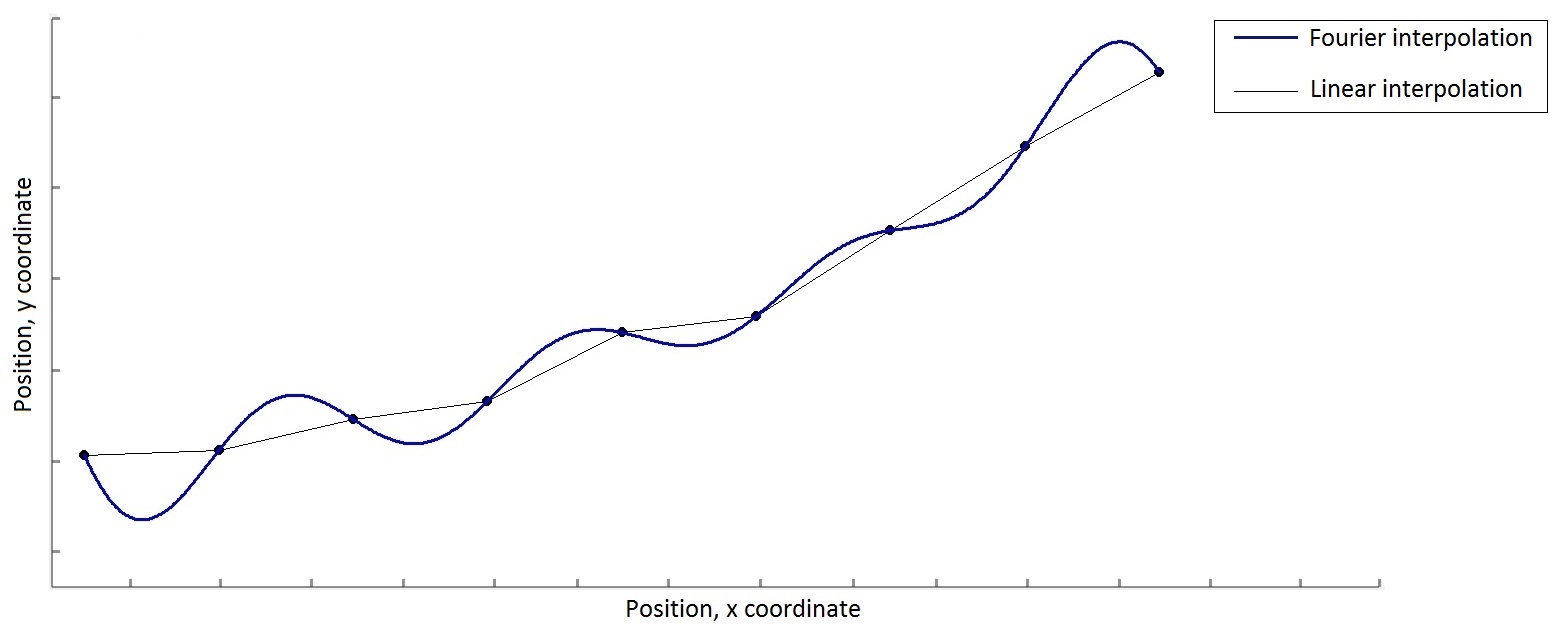
\includegraphics[width=11cm]{img/fourier.jpg}
\caption{Interpolation example with Fourier series.}
\label{fourier_fail}
\end{figure}

In \autoref{fourier_fail}, knot points come from a correction (in black) and it's Fourier series interpolation (in blue). The result Fourier curve is oscillating between the points, but still fitting them. This method adds wrong information in the trajectory. It doesn't represent then the correction.\\

\subsection{Non-linear regression with Taylor series}

By minimizing the error from discrete data to a $n^{th}$-order polynomial function, it's possible to interpolate data with a continuous and n-derivative function. This method fits well the knot points. It also keeps the general look of the curve without adding peak or high frequencies, see \autoref{taylor_graph}.

\begin{figure}[H]
\centering
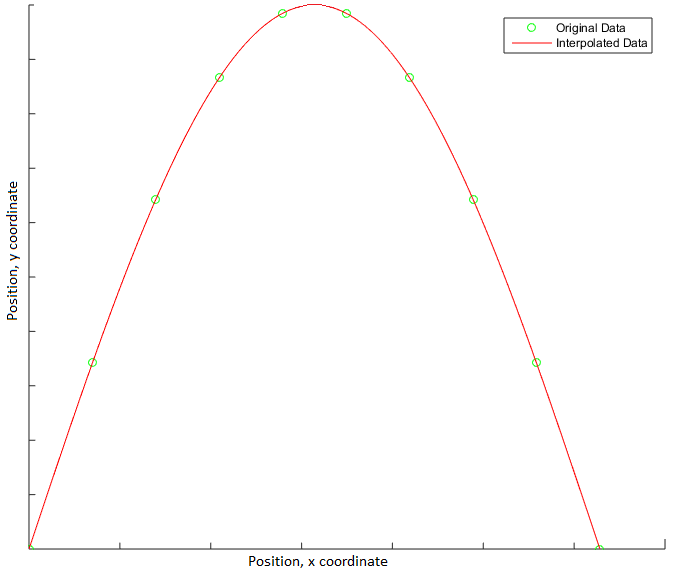
\includegraphics[width=10cm]{img/taylor.png}
\caption{Interpolation example of a $10^{th}$order polynomial function.}
\label{taylor_graph}
\end{figure}

\paragraph*{Advantage}

This method is quite fast to compute and represents well the correction. It provides a n-derivative form.

\paragraph*{Disadvantage}

There are no real disadvantage for this method, only one: this method is not compatible for an analytic distance resolution (which is presented in Continuous Gaussian process regression (\ref{GPR_ANALYTIC_SUBSUB}) ).

\clearpage

\subsection{B\'{e}zier curve}

A B\'{e}zier curve, also called B-Spline, is a parametric function which is often used in computer graphics.

\begin{figure}[H]
    \begin{minipage}[b]{0.5\linewidth}
        \centering
        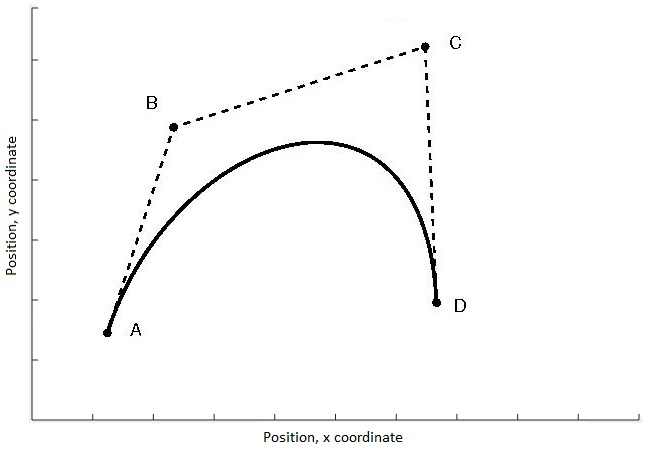
\includegraphics[width=7cm]{img/bspline.jpg}
		\caption[Caption for LOF]{Interpolation example of a B-Spline.\footnotemark}
		\label{bezier_example}
    \end{minipage}
    \begin{minipage}[b]{0.5\linewidth}
        \centering 
        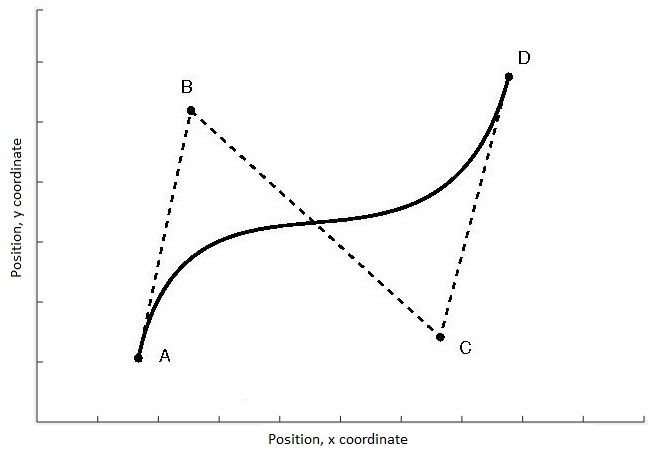
\includegraphics[width=7cm]{img/bspline2.jpg}
		\caption[Caption for LOF]{$2^{nd}$ interpolation example of a B-Spline.\footnotemark}
		\label{bezier_example2}
    \end{minipage}\hfill
\end{figure}

\footnotetext[1]{Found on: \url{http://pulsar.webshaker.net/2012/08/29/les-courbes-de-bezier-1/}}
\footnotetext[2]{Found on: \url{http://pulsar.webshaker.net/2012/08/29/les-courbes-de-bezier-1/}}

\paragraph*{Advantage}

This method returns a very smooth result which is, in our case, convenient as there could be some irregularities in the knot points.

\paragraph*{Disadvantage}

This method does not fit the points at all, the curve is not even going close to the testing points (see in \autoref{bezier_example} or \autoref{bezier_example2}).

\clearpage
\subsection{Spline}

A Spline is composed by a set of many parametric polynomial functions with a given order, cubic spline functions are commonly used in this case. With a cubic spline, it's not possible to fit an entire correction but only 2 position points. For this reason, one Spline is composed of many polynomial functions (called cubic splines), one between each couple of points, see \autoref{cubic_splines}.

\begin{figure}[H]
\centering
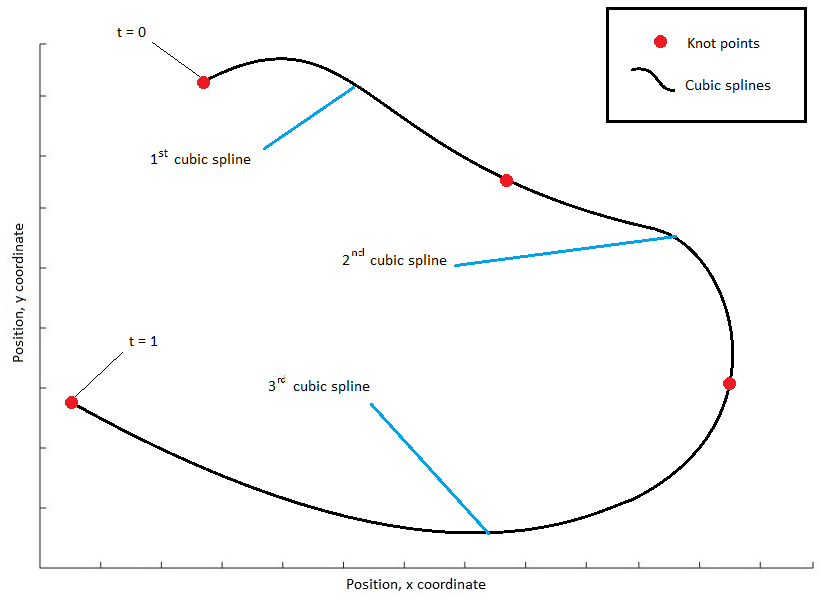
\includegraphics[width=13cm]{img/cubic_splines.png}
\caption{Example of spline interpolation with 4 knot points and 3 polynomial functions.}
\label{cubic_splines}
\end{figure}

In our application, the correction is in 3 dimensions. Therefore, there would be 3 Splines, one for each axis (and each spline is composed of many cubic splines). All would be parametrized by the same variable: $t\in[0,1]$ ($t$ goes from 0 to 1 over the entire correction, not on each polynomial function between points, see \autoref{cubic_splines})\\
There are many ways to compute the coefficient of the cubic splines that we will see.

\subsubsection{Position constraint}

It's possible to use natural cubic splines, it is the easiest and most common way to do it. Natural cubic splines $S(x)$ need to follow some properties:
\begin{itemize}  

        \item $S(x)$ should interpolate the position of all data points

        \item $S(x)$ should be continuous all along the curve

        \item $S'(x)$ should be continuous all along the curve

        \item $S''(x)$ should be continuous all along the curve

        \item For the first and the last points: $S''(x)=0$

\end{itemize}

Between every couple of points, in order to follow the 5 rules, there is a system to solve to get the coefficients of the polynomial functions. This is how natural splines are computed, see \autoref{Spline_interpolation_fig}. Indeed, with cubic splines it is very easy to follow the properties enunciate before:
\begin{equation}
\begin{split}
S(x) &= ax^3+bx^2+cx+d\\
S'(x) &= 3ax^2+2bx+c\\
S''(x) &= 6ax+2b
\end{split}
\end{equation}

\begin{figure}[H]
\centering
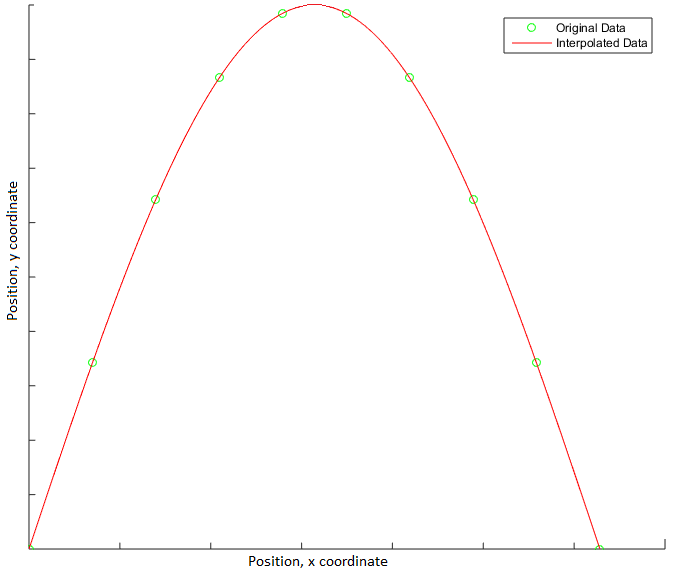
\includegraphics[width=10cm]{img/splines.png}
\caption{Interpolation example of cubic splines.}
\label{Spline_interpolation_fig}
\end{figure}

Spline allows a good fitting, fast computation time and it appear that the result is the same as the Taylor polynomial fitting. However, Splines and Taylor function are very different, both of them are a polynomial function but, almost all the time, with a different order. Taylor interpolation will be a $n^{th}$-order polynomial, where n is the number of points and cubic splines are third-order polynomials. To fit the knot points, a spline-interpolation is composed by many cubic spline functions.

\clearpage
\subsubsection{Position and velocity constraint}

Using cubic splines, it is also possible to compute it with the point's position and velocity. Indeed, By deriving the system (robots provide position and velocity for each point which very convenient in this case) it's possible to solve the system and get the coefficient of the polynomials function.\\
The properties will be: 
\begin{itemize}  

        \item $S(x)$ should interpolate the position of all data points

        \item $S(x)$ should be continuous all along the curve

        \item $S'(x)$ should interpolate the derivative of all data points

        \item $S'(x)$ should be continuous all along the curve

\end{itemize}
Those conditions are enough to compute the splines.\\
The curve will be composed by one cubic spline between each point (indeed each data point carries either a position and a velocity).

\paragraph*{Advantage}

Fitting the position and the velocity gives, with small computation time, the best fit. Indeed, fitting both position and derivative of the position is important for a good continuity of the curve.

\paragraph*{Disadvantage}

Constraining both position and velocity over-constraint the curve. Sometimes, non-expected results appear, see \autoref{splines_bad}.\\
In the following graph, each dimension interpolated over a t variable, therefore there 3 Splines.

\begin{figure}[H]
\centering
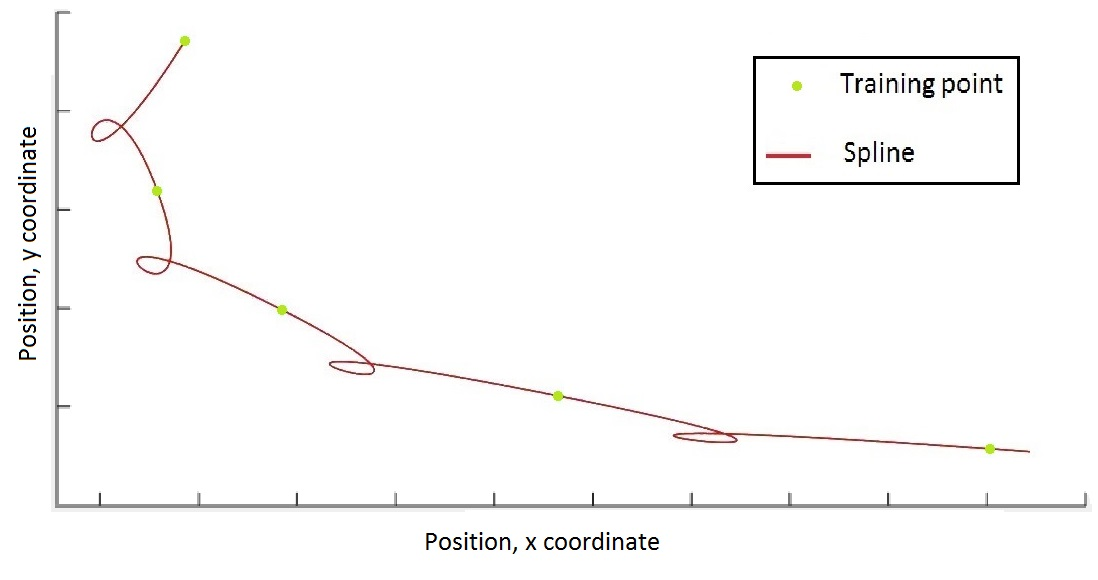
\includegraphics[width=13cm]{img/splines_bad.jpg}
\caption{Interpolation example of a problematic over-constraint cubic Spline.}
\label{splines_bad}
\end{figure}

The spline interpolation created some very small loops, this is an effect of over-constraining. This case needs to be avoid because the goal of the curve fitting is to provide clean data, not dirtier data.

\subsection{Method chosen}

Fourier interpolation could be chosen, but for complexity and general representation of the aspect of the curve this solution wasn't chosen. Furthermore this solution is not compatible for the future distance algorithm.\\
B-splines do not fit the points which makes the solution interesting for smoothing reason but not usable in our application.\\
Taylor polynomials is a very good method, but for the future distance algorithm reason, splines are better. \\
Splines give good results, when constraining them with velocity, some loops appear which is not acceptable, but basic spline (position fitting) is the best method to represent a correction, this method is chosen for next steps.

